\chapter{Design strategies}
We implemented a number of strategies for improving efficiency of raSAT: incremental search and refinement heuristics.
\section{Incremental search} \label{sec:incsearch}
{\bf raSAT} applies three incremental strategies, 
(1) {\em incremental windening}, (2) {\em incremental deepening} and (3) {\em incremental testing}. 
Let
$F = \exists x_1 \in I_1 \cdots x_n \in I_n. \bigwedge \limits_{j=1}^m f_j > 0$
for $I_i = (a_i,b_i)$. %where $a_i, b_i$ would be $\pm \infty$. 

\subsection{Incremental windening}
Given $0 < \delta_0 < \delta_1 < \cdots$, 
{\em incremental windening} starts with 
$F_0 = \exists x_1 \in I_1 \cap (-\delta_0 , \delta_0) \cdots x_n \in I_n \cap (-\delta_0 , \delta_0). 
\bigwedge \limits_{j=1}^m f_j > 0$, 
and if it finishes with UNSAT, it runs with 
$F_1 = \exists x_1 \in I_1 \cap (-\delta_1 , \delta_1) \cdots x_n \in I_n \cap (-\delta_1 , \delta_1). 
\bigwedge \limits_{j=1}^m f_j > 0$, and so on (Fig.~\ref{fig:incwid} (a)). 

Note that if $\delta_i < \infty$, {\bf raSAT} applies an Affine interval; otherwise, 
it uses CI. 
Experiments in Section~\ref{sec:experiment} are performed 
with $\delta_0 = 10$ and $\delta_1 = \infty$.
\begin{figure}[ht]
\begin{minipage}[b]{1.0\linewidth}
\centering
\begin{tabular}{c@{\qquad}c}
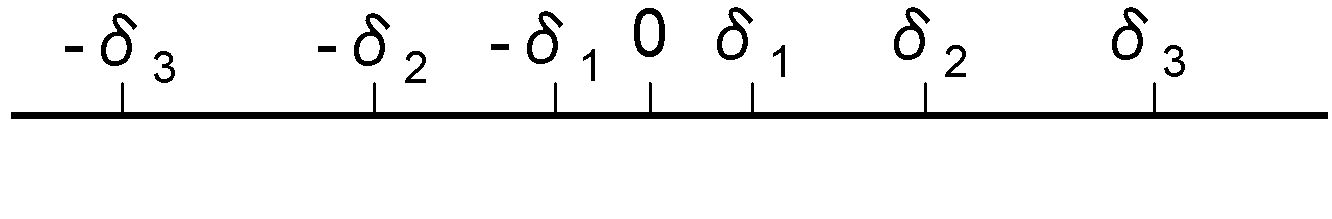
\includegraphics[height=0.4in,width=1.8in]{IncWiden.png} &
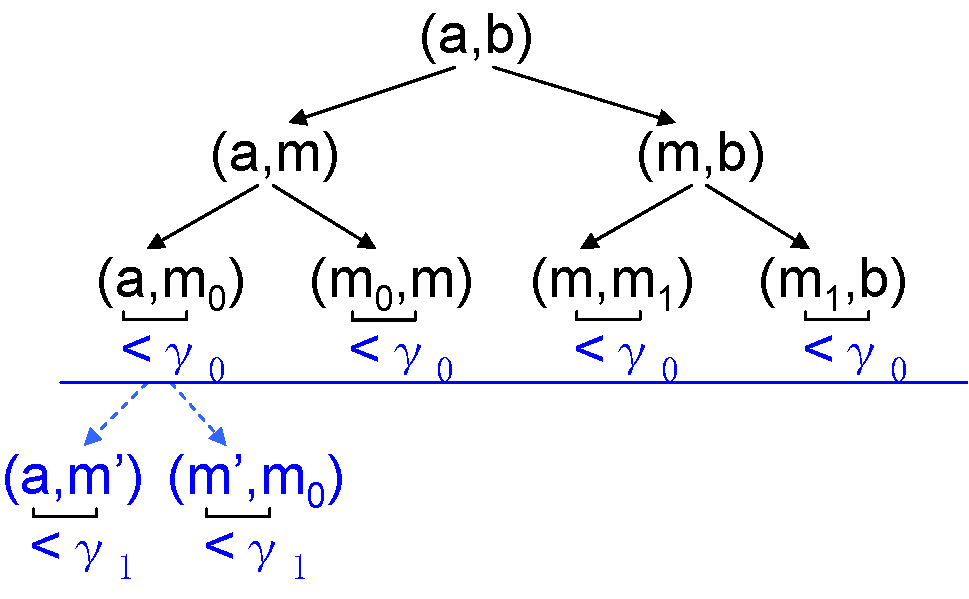
\includegraphics[height=1.2in,width=2in]{IncDeepen.png} \\
\mbox{(a) Incremenal widening} & \mbox{(b) Incremental Deepening} \\
\end{tabular}
\caption{Incremental Widening and Deepening}
\label{fig:incwid}
\end{minipage}
\end{figure}


\subsection{Incremental deepening}

Starting with $F = \exists x_1 \in I_1 \cdots x_n \in I_n. \bigwedge \limits_{j=1}^m f_j > 0$, 
$I_1 \times \cdots \times I_n$ is decomposed into many boxes, 
and $F$ becomes the disjunction of existential formulae corrsponding to these boxes. 
{\bf raSAT} searches these boxes in depth-first manner. Figure \ref{fig:depth-first-search} illustrates the search procedure of raSAT. First, the initially box $I$ is examined (by IA and testing) and suppose raSAT detects neither SAT or UNSAT here. As a consequence, $I$ is decomposed into $2$ boxes $I_{11}$ and $I_{12}$ such that $\bar{x} \in I \leftrightarrow \bar{x} \in I_{11} \vee \bar{x} \in I_{12}$. raSAT will choose one of the two boxes to explore, for example $I_{11}$. If IA and testing cannot detect satisfiability of the given constraint in the box $I_{11}$, decomposition of this box takes place:  $\bar{x} \in I_{11} \leftrightarrow \bar{x} \in I_{21} \vee \bar{x} \in I_{22}$. Either $I_{21}$ or $I_{22}$ is selected next. The process continues until SAT/UNSAT is detected which may leads to exhaustive local search.
To avoid it, {\bf raSAT} applies a threshold $\gamma$, such that no more decomposition will be 
applied when a box becomes smaller than $\gamma$. 
If neither SAT nor UNSAT is detected, {\bf raSAT} restarts with a smaller threshold. 

Let $\gamma_0 > \gamma_1 > \cdots > 0$, and {\bf raSAT} incrementally deepens its search 
with these thresholds, i.e., starting with $\delta_0$, and if it fails, restart with $\delta_1$, 
and so on (Fig~\ref{fig:incwid} (b)). 

\begin{comment}

\begin{figure}[ht]
%\begin{minipage}[b]{1.0\linewidth}
\centering
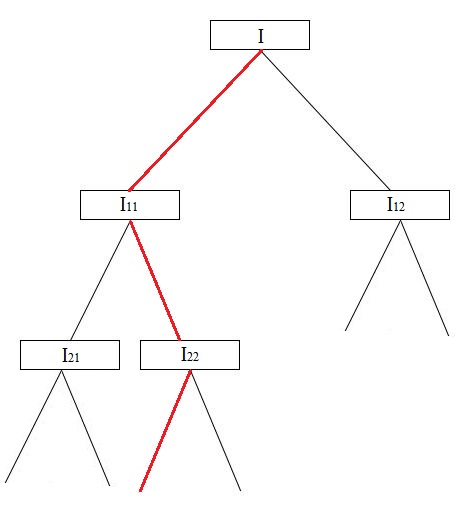
\includegraphics{depth-first-search.jpg} 
\caption{\textbf{raSAT} design} 
\label{fig:depth-first-search} 
%\end{minipage}
\end{figure} 
\end{comment}
\subsection{Incremental testing}
One obstacle in testing is the exponentially large number of test instances. If $2$ values are generated for each of $n$ variables, $2^n$ test cases (combinations of generated values) will present. 
\begin{example}
Suppose $\{x, y\}$ is the set of variables which appears in the input constraint and let $\{2, 9\}$ and $\{5, 8\}$ are generated values for $x$ and $y$ respectively. In total $4$ test cases arise: $(x, y) = (2, 5), (2, 8), (9, 5), (9, 8)$.
\end{example}

In order to tackle the problem, the following strategies are proposed:
\begin{enumerate}
\item Restrict the number of test cases to $2^{10}$ by choosing most $10$ influential variables which are decided by the following procedures for generating multiple ($2$) test values.
\begin{itemize}
\item Select API by SAT-likelihood
\item Select $1$ variable of each selected API.
\end{itemize}
\item Incrementally generate test values for variables to prune test cases that do not satisfy an API. This was proposed by \citeauthor{khanhReport} in \cite{khanhReport}:
\begin{itemize}
\item Dynamically sort the IA-SAT APIs.
\item Generate the test values for variables of selected APIs.
\end{itemize}
\begin{example}
Let $x^2 > 4$ and $x*y > 0$ are two IA-VALID APIs to be tested and somehow they are sorted in that order, i.e. $x^2 > 4$ is selected before $x*y > 0$. Suppose $\{1, 3\}$ are generated as test values for $x$ which are is enough to test the first selected API, i.e. $x^2 > 4$. As a result of testing, $x = 1$ is excluded from the satisfiable test cases whilst $x = 3$ is not. Next, when $x*y > 0$ is considered, $y$ needs to be generated $2$ values, e.g. $\{-3, 4\}$ and two test cases $(x, y) = (3, -3), (3, 4)$ come out to be checked. In this example, $(x, y) = (1, -3)$ and  $(x, y) = (1, 4)$ are early pruned by only testing $x = 1$ against $x^2 > 4$ .
\end{example}
\begin{figure}[ht]
\centering
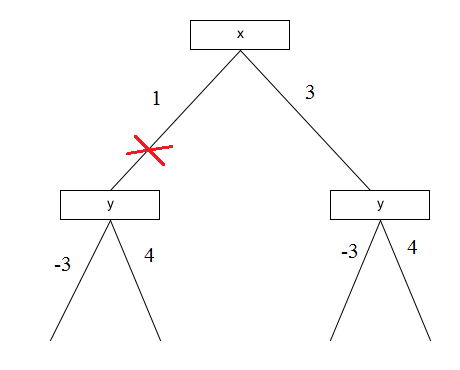
\includegraphics{incremental_test.png} 
\caption{Incremental Testing Example} 
\label{fig:incremental-test} 
%\end{minipage}
\end{figure} 
\end{enumerate}

\section{SAT directed heuristics measure} \label{sec:SATheuristics}

With several hundred variables, we observe that an SMT solver works 
when either SAT, or UNSAT with small UNSAT core.
%
For the latter, we need an efficient heuristics to find an UNSAT core, which is left as future work. 
For the former, the keys are how to choose variables to decompose, and 
how to choose a box to explore. 
{\bf raSAT} chooses such a variable in two steps; first it selects a {\em test-UNSAT API}, and
then chooses a variable that appears in the API. 
We design SAT-directed heuristic measures based on the interval arithemtic ($O.T$). 

Let $F = \exists x_1 \in I_1 \cdots x_n \in I_n. \bigwedge \limits_{j=1}^m f_j > 0$ 
becomes $\vee~( \exists x_1 \in I'_1 \cdots x_n \in I'_n. \bigwedge \limits_{j=1}^m f_j > 0)$ 
after box decomposition. 
For $\exists x_1 \in I'_1 \cdots x_n \in I'_n. \bigwedge \limits_{j=1}^m f_j > 0$, 
if some $f_j > 0$ is UNSAT, the box $I'_1 \times \cdots \times I'_n$ is UNSAT. 
If every $f_j > 0$ is SAT, $F$ is SAT. 
Thus, if the box $I'_1 \times \cdots \times I'_n$ needs to be explore, it must contain 
a test-UNSAT API (thus IA-SAT). 

We denote the estimated range of $f_j$ for $x_1 \in I'_1 \cdots x_n \in I'_n$ with IA ($O.T$)
by $range(f_j, I'_1 \times \cdots \times I'_n)$. 
If an IA is an affine interval, 
it is in the form $[c_1,d_1]\epsilon_1 + \cdots + [c_n,d_n]\epsilon_n$, 
and by instanciating $\epsilon_i$ with $[-1,1]$, 
the resulting classical interval coincides with $range(f_j, I'_1 \times \cdots \times I'_n)$. 
We define 
\begin{itemize} 
\item {\em Sensitivity} of a variable $x_i$ in a test-UNSAT API $f_j > 0$ is $max(|c_i|, |d_i|)$. 
\item {\em SAT-likelyhood} of an API $f_j > 0$ is $| I \cap (0,\infty) | / |I|$, and 
\item {\em SAT-likelyhood} of a box $I'_1 \times \cdots \times I'_n$ is 
the least SAT-likelyhood of test-UNSAT APIs. 
\end{itemize} 

\begin{example} \label{examp:SATlikelyhood}
In Example~\ref{examp:sensitivity}, 
\begin{itemize}
\item sensitivity is estimated $1$ for $x$ and $2$ for $y$ by $AF_2$, and $3\frac{1}{4}$ for $x$ and 
$2$ for $y$. 
\item SAT-likelyhood of $f$ is estimated $0.4= \frac{6}{9-(-6)}$ by $AF_2$ 
and $0.36 = \frac{4.5}{4.5-(-8)}$ by $CAI$. 
\end{itemize}
\end{example}


{\em SAT-likelyhood} intends to estimate APIs how likely to be SAT. 
For choosing variables, {\bf raSAT} first choose a test-UNSAT API by SAT-likelyhood. 
There are two choices, either {\em the largest} or {\em the least}. 
{\em Sensitivity} of a variable intends to estimate how a variable is influencial to the value of an API. 
From a selected API by SAT-likelyhood, {\bf raSAT} selects a variable with the largest sensitivity. 
This selection of variables are used for (1) {\em multiple test instances generation}, and 
(2) {\em decomposition}. 
For test generation, we will select multiple variables by repeating the selection. 

For choosing a box to explore, {\bf raSAT} chooses more likely to be SAT. 
There are two choice, (1) a box with the largest SAT-likelyhood, and 
(2) a box with the largest number of SAT (either IA-valid or test-SAT) APIs.

\section{Other}
UNSAT core, test case generation, interval decomposition 